\chapter{Экспериментальная часть}

В данном разделе описана параметризация реализации муравьиного алгоритма,  проведённые замеры и представлены результаты исследования. Также будут уточнены характеристики устройства, на котором проводились замеры.

\section{Технические характеристики}
Технические характеристики устройства, на котором выполнялось тестирование \cite{item4}:
\begin{itemize}
	\item операционная система $macOS$ $Monterey$ 12.4;
	\item 8 ГБ оперативной памяти;
	\item процессор $Apple$ $M2$ (базовая частота~---~2400 МГц, но поддержка технологии $Turbo$ $Boost$ позволяет достигать частоты в 3500 МГц \cite{item5}).
\end{itemize}

\section{Параметризация реализации муравьиного алгоритма}
Целью проведения параметризации является определение таких сочетаний входных параметров, при которых алгоритм даёт наилучшие и стабильные результаты.
В результате параметризации получена таблица со следующими столбцами:
\begin{itemize}
	\item $\alpha$~---~коэффициент стадности;
	%\item $\beta$~---~коэффициент жадности;
	\item $time$~---~количество дней жизни колонии;
	\item $ideal$~---~результат работы алгоритма полного перебора;
	\item $diff$~---~погрешность муравьиного алгоритма.
\end{itemize}

Параметризация проведена для трёх графов городов Африки, составленных по указанным выше принципам.

\subsection{Параметризация для графа №1}
Матрица смежности для графа №1 имеет следующий вид:
\begin{equation}
	\begin{pmatrix}
		0 & 525 & 907 & 1639\\
		525 & 0 & 606 & 965\\
		907 & 606 & 0 & 357\\
		1639 & 965 & 357 & 0
	\end{pmatrix}.
\end{equation}

В таблице \ref{table:par1} приведена усечённая выборка параметров, которые наилучшим образом решают поставленную задачу, что значит, что отсутствует погрешность относительно идеального результата.

\begin{table}[H]
  \caption{\label{table:par1} Результаты параметризующего запуска для графа №1 из 4 вершин}
  \begin{center}
    \begin{tabular}{
    |S[table-format=5.2]
    |S[table-format=5.2]
    |S[table-format=5.2]
    |S[table-format=5.2]
    |S[table-format=5.2]
    |S[table-format=5.2]|
    }
      \hline
      {$\alpha$} & {$\beta$} & {$\rho$} & {$time$} & {$ideal$} & {$diff$} \\ \hline
      0.1 & 0.9 & 0.1 & 1 & 2754 & 0 \\ \hline 
0.1 & 0.9 & 0.1 & 2 & 2754 & 0 \\ \hline 
0.1 & 0.9 & 0.1 & 3 & 2754 & 0 \\ \hline 
0.1 & 0.9 & 0.2 & 1 & 2754 & 0 \\ \hline 
0.1 & 0.9 & 0.2 & 2 & 2754 & 0 \\ \hline
0.3 & 0.7 & 0.6 & 1 & 2754 & 0 \\ \hline 
0.3 & 0.7 & 0.6 & 2 & 2754 & 0 \\ \hline 
0.3 & 0.7 & 0.6 & 3 & 2754 & 0 \\ \hline
0.4 & 0.6 & 0.1 & 1 & 2754 & 0 \\ \hline 
0.4 & 0.6 & 0.1 & 2 & 2754 & 0 \\ \hline 
0.4 & 0.6 & 0.1 & 3 & 2754 & 0 \\ \hline 
0.4 & 0.6 & 0.2 & 1 & 2754 & 0 \\ \hline 
0.4 & 0.6 & 0.2 & 2 & 2754 & 0 \\ \hline
0.5 & 0.5 & 0.2 & 3 & 2754 & 0 \\ \hline 
0.5 & 0.5 & 0.3 & 1 & 2754 & 0 \\ \hline 
0.5 & 0.5 & 0.3 & 2 & 2754 & 0 \\ \hline 
0.5 & 0.5 & 0.3 & 3 & 2754 & 0 \\ \hline 
0.5 & 0.5 & 0.4 & 1 & 2754 & 0 \\ \hline 
0.5 & 0.5 & 0.4 & 2 & 2754 & 0 \\ \hline
0.8 & 0.2 & 0.3 & 1 & 2754 & 0 \\ \hline 
0.8 & 0.2 & 0.3 & 2 & 2754 & 0 \\ \hline
%0.1 & 0.1 & 0.2 & 3 & 2754 & 0 \\ \hline 
%0.1 & 0.1 & 0.3 & 1 & 2754 & 0 \\ \hline 
%0.1 & 0.1 & 0.3 & 2 & 2754 & 0 \\ \hline 
%0.1 & 0.1 & 0.3 & 3 & 2754 & 0 \\ \hline 
%0.1 & 0.1 & 0.4 & 1 & 2754 & 0 \\ \hline 
%0.3 & 1.0 & 1.0 & 1 & 2754 & 0 \\ \hline 
%0.3 & 1.0 & 1.0 & 2 & 2754 & 0 \\ \hline 
%0.3 & 1.0 & 1.0 & 3 & 2754 & 0 \\ \hline 
%0.4 & 0.1 & 0.1 & 1 & 2754 & 0 \\ \hline 
%0.4 & 0.1 & 0.1 & 2 & 2754 & 0 \\ \hline 
%0.4 & 0.1 & 0.1 & 3 & 2754 & 0 \\ \hline 
%0.4 & 0.1 & 0.2 & 1 & 2754 & 0 \\ \hline 
%0.4 & 0.1 & 0.2 & 2 & 2754 & 0 \\ \hline
%0.5 & 0.4 & 0.8 & 2 & 2754 & 0 \\ \hline  
%0.5 & 0.4 & 1.0 & 1 & 2754 & 0 \\ \hline 
%0.5 & 0.4 & 1.0 & 2 & 2754 & 0 \\ \hline 
%0.5 & 0.4 & 1.0 & 3 & 2754 & 0 \\ \hline 
%0.5 & 0.5 & 0.1 & 1 & 2754 & 0 \\ \hline 
%0.5 & 0.5 & 0.1 & 2 & 2754 & 0 \\ \hline 
%0.8 & 0.4 & 0.9 & 1 & 2754 & 0 \\ \hline 
%0.8 & 0.4 & 0.9 & 2 & 2754 & 0 \\ \hline
    \end{tabular}
  \end{center}
\end{table}

\subsection{Параметризация для графа №2}
Матрица смежности для графа №2 имеет следующий вид:
\begin{equation}
	\begin{pmatrix}
		0 & 525 & 907 & 1639 & 2346 & 5141 & 4123 & 945\\
		525 & 0 & 606 & 965 & 1789 & 4728 & 3879 & 1370\\
		907 & 606 & 0 & 357 & 1221 & 4095 & 3421 & 1649\\
		1639 & 965 & 357 & 0 & 885 & 3757 & 3172 & 1874\\
		2346 & 1789 & 1221 & 885 & 0 & 2631 & 2263 & 2221\\
		5141 & 4728 & 4095 & 3757 & 2631 & 0 & 1223 & 4384\\
		4123 & 3879 & 3421 & 3172 & 2263 & 1223 & 0 & 3253\\
		945 & 1370 & 1649 & 1874 & 2221 & 4384 & 3253 & 0\\
	\end{pmatrix}.
\end{equation}

В таблице \ref{table:par2} приведена усечённая выборка параметров, которые наилучшим образом решают поставленную задачу, что значит, что отсутствует погрешность относительно идеального результата.

\begin{table}[H]
  \caption{\label{table:par2} Результаты параметризующего запуска для графа №2 из 8 вершин}
  \begin{center}
    \begin{tabular}{
    |S[table-format=5.2]
    |S[table-format=5.2]
    |S[table-format=5.2]
    |S[table-format=5.2]
    |S[table-format=5.2]
    |S[table-format=5.2]|
    }
      \hline
      {$\alpha$} & {$\beta$} & {$\rho$} & {$time$} & {$ideal$} & {$diff$} \\ \hline 
      0.1 & 0.9 & 0.3 & 1 & 10425 & 0 \\ \hline 
0.1 & 0.9 & 0.3 & 2 & 10425 & 0 \\ \hline 
0.1 & 0.9 & 0.3 & 3 & 10425 & 0 \\ \hline
0.2 & 0.8 & 0.6 & 2 & 10425 & 0 \\ \hline 
0.2 & 0.8 & 0.6 & 3 & 10425 & 0 \\ \hline 
0.2 & 0.8 & 0.7 & 1 & 10425 & 0 \\ \hline
0.6 & 0.4 & 0.1 & 2 & 10425 & 0 \\ \hline 
0.6 & 0.4 & 0.1 & 3 & 10425 & 0 \\ \hline 
0.6 & 0.4 & 0.2 & 1 & 10425 & 0 \\ \hline
0.7 & 0.3 & 0.1 & 2 & 10425 & 0 \\ \hline 
0.7 & 0.3 & 0.1 & 3 & 10425 & 0 \\ \hline 
0.7 & 0.3 & 0.2 & 1 & 10425 & 0 \\ \hline
0.8 & 0.2 & 0.2 & 3 & 10425 & 0 \\ \hline 
0.8 & 0.2 & 0.3 & 1 & 10425 & 0 \\ \hline
1.0 & 0.0 & 0.4 & 3 & 10425 & 0 \\ \hline 
1.0 & 0.0 & 0.5 & 1 & 10425 & 0 \\ \hline 
1.0 & 0.0 & 0.5 & 2 & 10425 & 0 \\ \hline
%0.1 & 0.1 & 0.8 & 1 & 10425 & 0 \\ \hline 
%0.1 & 0.1 & 0.8 & 2 & 10425 & 0 \\ \hline 
%0.1 & 0.1 & 0.8 & 3 & 10425 & 0 \\ \hline 
%0.2 & 0.9 & 0.5 & 3 & 10425 & 0 \\ \hline 
%0.2 & 0.9 & 0.6 & 1 & 10425 & 0 \\ \hline  
%0.2 & 0.9 & 0.6 & 3 & 10425 & 0 \\ \hline  
%0.6 & 0.3 & 0.2 & 2 & 10425 & 0 \\ \hline 
%0.6 & 0.3 & 0.2 & 3 & 10425 & 0 \\ \hline 
%0.6 & 0.3 & 0.3 & 1 & 10425 & 0 \\ \hline 
%0.7 & 0.1 & 0.8 & 3 & 10425 & 0 \\ \hline  
%0.7 & 0.1 & 0.9 & 2 & 10425 & 0 \\ \hline 
%0.7 & 0.1 & 0.9 & 3 & 10425 & 0 \\ \hline  
%0.8 & 0.9 & 0.1 & 2 & 10425 & 0 \\ \hline 
%0.8 & 0.9 & 0.1 & 3 & 10425 & 0 \\ \hline  
%1.0 & 0.9 & 0.6 & 1 & 10425 & 0 \\ \hline 
%1.0 & 0.9 & 0.6 & 2 & 10425 & 0 \\ \hline 
%1.0 & 0.9 & 0.6 & 3 & 10425 & 0 \\ \hline
    \end{tabular}
  \end{center}
\end{table}

\subsection{Параметризация для графа №3}
Матрица смежности для графа №3 имеет следующий вид:
\begin{equation}
	\begin{pmatrix}
		0 & 525 & 907 & 1639 & 2346 & 5141 & 4123 & 945 & 1327 & 1970\\
		525 & 0 & 606 & 965 & 1789 & 4728 & 3879 & 1370 & 899 & 1655\\
		907 & 606 & 0 & 357 & 1221 & 4095 & 3421 & 1649 & 1237 & 1290\\
		1639 & 965 & 357 & 0 & 885 & 3757 & 3172 & 1874 & 1318 & 1129\\
		2346 & 1789 & 1221 & 885 & 0 & 2631 & 2263 & 2221 & 1465 & 1024\\
		5141 & 4728 & 4095 & 3757 & 2631 & 0 & 1223 & 4384 & 3445 & 2588\\
		4123 & 3879 & 3421 & 3172 & 2263 & 1223 & 0 & 3253 & 2408 & 1760\\
		945 & 1370 & 1649 & 1874 & 2221 & 4384 & 3253 & 0 & 795 & 1597\\
		1327 & 899 & 1237 & 1318 & 1465 & 3445 & 2408 & 795 & 0 & 1028\\
		1970 & 1655 & 1290 & 1129 & 1024 & 2588 & 1760 & 1597 & 1028 & 0
	\end{pmatrix}.
\end{equation}

В таблице \ref{table:par3} приведена усечённая выборка параметров, которые наилучшим образом решают поставленную задачу, что значит, что отсутствует погрешность относительно идеального результата.

\begin{table}[H]
  \caption{\label{table:par3} Результаты параметризующего запуска для графа №3 из 10 вершин}
  \begin{center}
    \begin{tabular}{
    |S[table-format=5.2]
    |S[table-format=5.2]
    |S[table-format=5.2]
    |S[table-format=5.2]
    |S[table-format=5.2]
    |S[table-format=5.2]|
    }
      \hline
      {$\alpha$} & {$\beta$} & {$\rho$} & {$time$} & {$ideal$} & {$diff$} \\ \hline 
      0.1 & 0.9 & 0.5 & 3 & 10755 & 0 \\ \hline 
0.1 & 0.9 & 0.6 & 1 & 10755 & 0 \\ \hline
0.2 & 0.8 & 0.1 & 3 & 10755 & 0 \\ \hline
0.3 & 0.7 & 1.0 & 2 & 10755 & 0 \\ \hline
0.4 & 0.6 & 0.2 & 2 & 10755 & 0 \\ \hline 
0.4 & 0.6 & 0.2 & 3 & 10755 & 0 \\ \hline
0.5 & 0.5 & 0.7 & 3 & 10755 & 0 \\ \hline
0.6 & 0.4 & 0.1 & 2 & 10755 & 0 \\ \hline
0.7 & 0.3 & 0.1 & 2 & 10755 & 0 \\ \hline 
0.7 & 0.3 & 0.1 & 3 & 10755 & 0 \\ \hline
0.8 & 0.2 & 0.1 & 2 & 10755 & 0 \\ \hline 
0.8 & 0.2 & 0.1 & 3 & 10755 & 0 \\ \hline
0.9 & 0.1 & 0.5 & 3 & 10755 & 0 \\ \hline
0.9 & 0.1 & 1.0 & 2 & 10755 & 0 \\ \hline 
0.9 & 0.1 & 1.0 & 3 & 10755 & 0 \\ \hline
%0.1 & 0.1 & 0.1 & 2 & 10755 & 0 \\ \hline 
%0.1 & 0.1 & 0.1 & 3 & 10755 & 0 \\ \hline 
%0.2 & 0.4 & 0.6 & 2 & 10755 & 0 \\ \hline  
%0.3 & 0.3 & 0.7 & 2 & 10755 & 0 \\ \hline  
%0.4 & 0.2 & 0.7 & 1 & 10755 & 0 \\ \hline 
%0.4 & 0.2 & 0.7 & 2 & 10755 & 0 \\ \hline  
%0.5 & 0.5 & 0.7 & 3 & 10755 & 0 \\ \hline  
%0.6 & 0.1 & 0.5 & 3 & 10755 & 0 \\ \hline  
%0.7 & 0.2 & 0.3 & 3 & 10755 & 0 \\ \hline   
%0.7 & 0.8 & 0.1 & 2 & 10755 & 0 \\ \hline 
%0.8 & 0.2 & 0.5 & 1 & 10755 & 0 \\ \hline 
%0.8 & 0.2 & 0.5 & 2 & 10755 & 0 \\ \hline   
%0.9 & 0.2 & 0.8 & 2 & 10755 & 0 \\ \hline  
%1.0 & 0.3 & 0.6 & 2 & 10755 & 0 \\ \hline 
%1.0 & 0.3 & 0.6 & 3 & 10755 & 0 \\ \hline
    \end{tabular}
  \end{center}
\end{table}

\section{Измерение времени выполнения реализаций алгоритмов}
Замеры времени реализаций алгоритмов производилось при помощи импортируемой в $Go$ функции $clock\_gettime$ языка $C$ \cite{item15}. Эта функция при использовании макроса \\ $CLOCK\_PROCESS\_CPUTIME\_ID$ возвращает затраченное на работу процесса процессорное время в формате структуры $struct\ timespec$, в которой хранятся результаты замеров из двух частей~---~в секундах и наносекундах (см. листинг \ref{code:timespec}).

\begin{code}
\caption{Листинг структуры $struct\ timespec$}
\label{code:timespec}

\begin{minted}{c}
struct timespec {
	time_t   tv_sec;        /* seconds */
	long     tv_nsec;       /* nanoseconds */
};
\end{minted}
\end{code}

Количество повторений замера для одинаковых входных данных~---~100.

Функция, возвращающая текущее процессорное время, приведена в листинге \ref{code:cpu}.

\begin{code}
\caption{Листинг функции, возвращающей текущее процессорное время}
\label{code:cpu}

\begin{minted}{c}
#include <pthread.h>
#include <time.h>
#include <stdio.h>

static long long getCPUNs(){
	struct timespec time;
	if (clock_gettime(CLOCK_PROCESS_CPUTIME_ID, &time)) {
		perror("can't measure time");
		return 0;
	}
	return time.tv_sec * 1000000000LL + time.tv_nsec;
}
\end{minted}
\end{code}

Функция единичного замера времени выполнения в наносекундах приведена в листинге \ref{code:measure} (в примере функция замеряет время работы реализации алгоритма полного перебора).

\newpage

\begin{code}
\caption{Листинг функции единичного замера времени выполнения в наносекундах}
\label{code:measure}
\begin{minted}{c}
func RunBenchmarkBF(g graph.Graph) int {
	t := 0

	start := C.getCPUNs()
	for i := 0; i < NumTests; i++ {
		bf.TravellingSalesmanBF(g)
	}
	end := C.getCPUNs()
	t = int(end-start) / NumTests

	return t
}
\end{minted}
\end{code}

Замеры проводились на графах, вершины которых представляют города Африки, а веса рёбер~---~расстояния между соответствующими городами. Вес ребра будет больше, если прямой путь между городами лежит через пустыню, и меньше, если пусть проходит через водоём (кроме рек).

В таблице \ref{table:total_time} представлены результаты замеров времени работы реализованных алгоритмов (в мкс.) при разном количестве вершин во входном графе, а на рисунке \ref{img:graph1} приведен график, отражающий зависимость времени выполнения реализаций решения задачи коммивояжёра от количества вершин во входном графе. В легендах графика и в таблице обозначение $ACO$ значит муравьиный алгоритм, а $BF$~---~алгоритм полного перебора.

\begin{table}[H]
  \caption{\label{table:total_time} Результаты замеров времени работы конвейера при разном количестве входных заявок (мкс.)}
  \begin{center}
    \begin{tabular}{
    |S[table-format=4.0]
    |S[table-format=10.0]
    |S[table-format=10.0]|
    }
      \hline
      {Кол-во вершин графа} & {ACO} & {BF} \\ \hline
      1 & 217 & 0\\ \hline
      2 & 912 & 0\\ \hline
      3 & 1780 & 0\\ \hline
      4 & 2987 & 1\\ \hline
      5 & 4371 & 19\\ \hline
      6 & 6114 & 51\\ \hline
      7 & 8068 & 377\\ \hline
      8 & 10531 & 6732\\ \hline
      9 & 13119 & 57514\\ \hline
      10 & 15990 & 622262\\ \hline
    \end{tabular}
  \end{center}
\end{table}

\noindent
\begin{table}[h!]
  \centering
  \begin{tabular}{p{1\linewidth}}
    \centering
    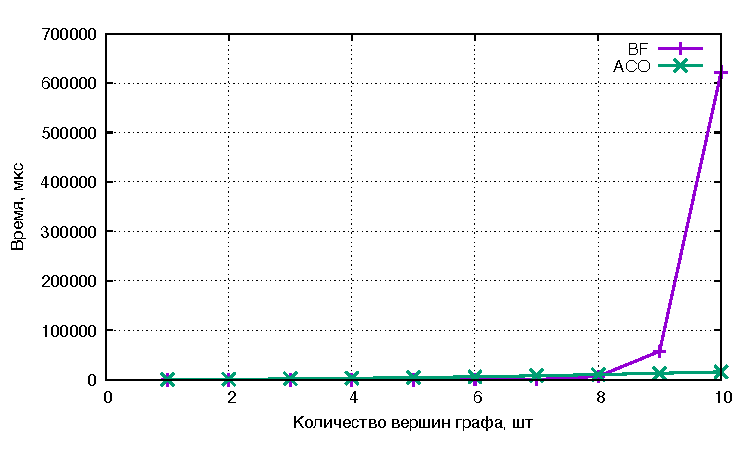
\includegraphics[width=0.8\linewidth]{./images/time.pdf}
    \captionof{figure}{Зависимость времени выполнения реализаций решения задачи коммивояжёра от количества вершин во входном графе}
    \label{img:graph1}
  \end{tabular}
\end{table}

\newpage